\chapter{Algoritmo genético}

\section{Evolución natural}

La evolución, en relación con la genómica, es el proceso por el cual los organismos vivos cambian con el tiempo a través de modificaciones en el genoma. Estos cambios provocan individuos con rasgos alterados que afectan su supervivencia. Los supervivientes se reproducen y transmiten estos genes alterados. Por otro lado, los cambios que atentan contra la supervivencia de un individuo impiden su reproducción \cite{evolucion}.

En la naturaleza, para que exista un proceso evolutivo se deben cumplir las siguientes condiciones:
\begin{itemize}
	\item Una entidad o individuo con la capacidad de reproducción.
	\item Una población de dichos individuos.
	\item Diferencias entre los individuos de la población.
	\item La variedad como factor determinante del nivel de supervivencia de cada individuo.
\end{itemize}

La evolución afecta a los cromosomas, que son estructuras encargadas de transportar la información genómica de una célula a otra. Es mediante la reproducción que se combinan los cromosomas de los padres para formar nuevas estructuras \cite{evolucion_2, cromosoma}.

\section{Evolución artificial}

Los algoritmos genéticos simulan el comportamiento evolutivo de una población, en la cual los más aptos heredan sus genes a las nuevas generaciones para obtener mejores resultados. Este proceso consta de los siguientes pasos:
\begin{itemize}
	\item \textbf{Selección}: Se seleccionan parejas (o grupos) de individuos de la población con las mejores aptitudes. Este conjunto será el encargado de generar la nueva generación.
	
	\item \textbf{Cruza}: Se realiza una combinación entre los genomas de las parejas seleccionadas para producir un número de hijos con códigos genéticos distintos.
	
	\item \textbf{Mutación}: Se realiza algún cambio aleatorio en el genoma de cualquier elemento de la nueva población.
	
	\item \textbf{Reemplazo}: Criterio que define qué elementos de la nueva generación reemplazarán a los de la generación anterior.
\end{itemize}

\subsection{Ventajas}

\begin{itemize}
	\item Pueden explorar el espacio de soluciones en múltiples direcciones simultáneamente.
	\item Realizan una exploración amplia, lo que permite escapar de óptimos locales para alcanzar óptimos globales.
	\item Funcionan bien en problemas complejos y dinámicos, así como en aquellos donde la función objetivo es discontinua, ruidosa o presenta múltiples óptimos locales. También permiten optimización multiobjetivo.
	\item Cada parte del proceso puede ser implementada con funciones específicas para mejorar el rendimiento del algoritmo; por ejemplo, existen funciones enfocadas únicamente en la exploración.
\end{itemize}

\subsection{Desventajas}

\begin{itemize}
	\item La función objetivo es muy sensible para los algoritmos genéticos; si se define incorrectamente, puede impedir encontrar una solución adecuada al problema.
	\item La elección de los parámetros (tamaño de la población, tasa de cruzamiento, selección de padres, tasa de mutación, entre otros) puede ser compleja. Una mala configuración puede provocar un bajo rendimiento.
	\item Requieren un alto tiempo de ejecución y potencia de cómputo.
	\item Existe el riesgo de convergencia prematura, es decir, que un individuo se reproduzca excesivamente y reduzca la diversidad genética, lo cual puede llevar a un óptimo local no deseado.
\end{itemize}

\subsection{Fenotipo y genotipo}

El \textbf{fenotipo} es la forma que toma la posible solución del problema, como números, cadenas, grafos, tablas, imágenes, etc. El \textbf{genotipo} (también llamado cromosoma) está construido a partir del fenotipo y representa la codificación de sus características, generalmente como un vector.

\begin{figure}[H]
	\centering
	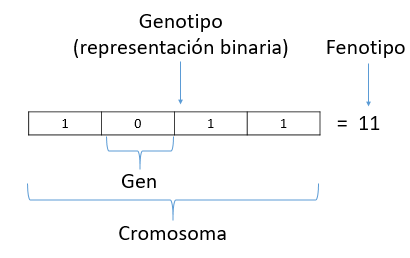
\includegraphics[width=0.75\linewidth]{img/fen_gen.png}
	\caption{Descripción gráfica de genotipo, fenotipo, cromosoma y gen del número ``11''}
	\label{fig:fen_gen}
\end{figure}

\subsection{Modelos generacionales y estacionarios}

En cada paso evolutivo, la cantidad de población seleccionada y la forma en que se reintegran los nuevos individuos afectan el comportamiento general de la población, la velocidad con la que evoluciona y el espacio de exploración en la búsqueda de óptimos globales.

Los \textbf{modelos generacionales} actualizan la mayor parte de la población. Buscan una evolución rápida y una amplia exploración. Para ello, se selecciona un pequeño conjunto de individuos y se les aplican los algoritmos de selección, cruza y mutación. Finalmente, mediante un algoritmo de reemplazo, se reintegran en la población mediante una función definida.

Por otro lado, los \textbf{modelos estacionarios} buscan mantener el equilibrio en la mayor parte de la población, experimentando y mezclando únicamente un pequeño subconjunto. El cambio es más lento, pero más estable.
